% FROST manuscript -- template-agnostic shell. Content lives in sections/*.tex.
\documentclass[11pt]{article}
\usepackage[margin=2.5cm]{geometry}
\usepackage[T1]{fontenc}
\usepackage{lmodern}
\usepackage{amsmath,amssymb,bm}
\usepackage{booktabs,multirow,array}
\usepackage{graphicx}
\usepackage[numbers,sort&compress]{natbib}
\usepackage{xr-hyper}
\usepackage[hidelinks]{hyperref}
\usepackage{xspace}
\usepackage{microtype}
\usepackage{tikz}
\usetikzlibrary{matrix}

\newcommand{\frost}{FROST\xspace}
\newcommand{\um}{\,\ensuremath{\mu}m\xspace}
\newcommand{\Cs}{\ensuremath{\mathbf{C}^{s}}\xspace}
\newcommand{\Ct}{\ensuremath{\mathbf{C}^{t}}\xspace}
\newcommand{\todo}[1]{\textbf{[TODO: #1]}}
\externaldocument[S-]{supplement}

\title{FROST: Reference-preserving post-hoc alignment of cross-platform spatial transcriptomics with fused Gromov--Wasserstein transport}
\author{}
\date{}

\begin{document}
\maketitle

\begin{abstract}
Spatial transcriptomics platforms differ in panel, resolution and chemistry, so serial sections of one tissue yield
cell embeddings that disagree across technologies. Most integration methods, including spatially aware ones,
re-embed all data jointly, which moves the reference and invalidates everything built on it. We present \frost, a
post-hoc method that maps cells from a source platform into a frozen reference embedding with fused
Gromov--Wasserstein transport. Building on USHER, \frost computes the structure matrices once rather than in every EM
iteration, fits a linear identity-regularised map and ends with closed-form moment matching. On SPATCH data (Xenium
5K reference; CosMx 6K, Visium HD FFPE, Visium HD FF and Stereo-seq sources; three tumour types; 12 pairs), \frost
ranks among the top three of 11 methods on seven summary metrics. It transfers labels more accurately than the
spatially aware GraphST (balanced accuracy 0.72 vs 0.37; exact Wilcoxon $p=0.0005$) with no significant difference
in mixing, whereas GraphST is worse than no alignment and displaces its own reference (neighbourhood drift 0.98;
zero for \frost by construction). Against the USHER reference implementation, \frost reaches a similar total score
from the other side of the mixing--conservation trade-off, with 25-fold fewer structure computations and about
7.5-fold less EM time. A global map fitted to distributions and labels does blur gene-level neighbourhoods: once
leakage is removed, imputation and neighbour-based deconvolution favour unaligned or locally corrected embeddings,
which defines the scope of the method.
\end{abstract}

\section{Introduction}\label{sec:intro}
Spatial transcriptomics platforms differ in almost every respect: imaging-based assays such as Xenium and CosMx
resolve single cells against targeted panels, while sequencing-based assays such as Visium HD and Stereo-seq capture
larger gene sets on grids. When serial sections of one tissue are profiled on several
platforms~\citep{ren2025spatch}, the same cell types land in different regions of an embedding space. Foundation
models~\citep{cui2024scgpt,wang2025scgptspatial,tejadalapuerta2025nicheformer} give every platform a common
vocabulary, but not a common geometry.

A common workflow annotates one high-quality reference and brings other data sets into it. Most integration
methods cannot support this. Harmony~\citep{korsunsky2019harmony}, Scanorama~\citep{hie2019scanorama} and spatially
aware methods such as GraphST~\citep{long2023graphst} return a new embedding for all inputs. The reference moves, and
every classifier, index or annotation built on it must be rebuilt. USHER~\citep{pratapa2025usher} instead keeps the
target fixed and learns a low-capacity map of the source into it, using fused Gromov--Wasserstein (FGW) transport to
find correspondences. Its structure matrices, however, are recomputed in every EM iteration, and this dominates its
run time. Because composite scores are dominated by batch mixing, which moment matching recovers cheaply, we read
results as a trade-off between mixing and conservation.

Our contributions are: (i) \frost, a post-hoc, reference-preserving FGW method whose structure matrices are built
once per batch ($2B$ rather than $2BT$ computations for $B$ batches and $T$ iterations) and which ends with
closed-form moment matching; (ii) a 12-pair benchmark across three tumour types and four source platforms against
ten baselines, with a measure of reference drift, in which a spatially aware integration method fails; (iii) a comparison with USHER showing similar total scores from opposite sides of the trade-off at
25-fold fewer structure computations at USHER's 25 EM iterations (a $T$-fold reduction for $T$ iterations); and (iv) a mechanistic account of why global alignment blurs gene-level
neighbourhoods, which sets the method's scope.

\section{Related work}\label{sec:related}
\paragraph{Joint integration.}
Harmony~\citep{korsunsky2019harmony}, Scanorama~\citep{hie2019scanorama} and mutual-nearest-neighbour
correction~\citep{haghverdi2018mnn} produce a new representation of all inputs, as do the spatially aware
GraphST~\citep{long2023graphst} and STAligner~\citep{zhou2023staligner}, which train graph encoders on all sections
jointly, so analyses built on the previous reference must be redone.

\paragraph{Mapping into a reference.}
Symphony~\citep{kang2021symphony} and scArches~\citep{lotfollahi2022scarches} map queries without changing the
reference, but the reference must be built in their own model rather than in an embedding the analyst already uses.
The lightest reference-preserving alternatives are affine or linear post-hoc adapters fitted after the fact: a
translation (mean centring), a second-order affine map (CORAL~\citep{sun2016coral}) or a linear map fitted on matched
cells; we include all three as baselines.

\paragraph{Optimal transport.}
SCOT~\citep{demetci2022scot} aligns modalities with Gromov--Wasserstein transport over $k$-NN geodesics. USHER~\citep{pratapa2025usher} couples
FGW correspondences with a low-capacity transform in an EM loop to move foundation-model embeddings into a fixed
target. \frost inherits this design and changes how and when the structure is computed.

\section{Methods}\label{sec:methods}

\subsection{Problem setting}\label{sec:setting}
Let $\mathbf{X}^{t}\in\mathbb{R}^{n_t\times d}$ be embeddings of annotated cells from a \emph{reference} platform
and $\mathbf{X}^{s}\in\mathbb{R}^{n_s\times d}$ embeddings of cells from the same tissue on a \emph{source}
platform. We learn $f_\theta:\mathbb{R}^{d}\to\mathbb{R}^{d}$ that places source cells in the reference coordinates while
$\mathbf{X}^{t}$ is never modified, so reference drift is zero by construction. Source labels are used only for
evaluation; spatial coordinates only within a section.

\subsection{Base algorithm: USHER}\label{sec:usher}
USHER~\citep{pratapa2025usher} alternates between correspondences and a transform. The E-step solves the FGW
problem~\citep{vayer2019fgw}
\begin{equation}\label{eq:fgw}
  \mathbf{P}^{\star}=\arg\min_{\mathbf{P}\in\Pi}\;(1-\alpha)\,\langle \mathbf{M},\mathbf{P}\rangle
  +\alpha\sum_{i,k,j,\ell}\bigl(C^{s}_{ik}-C^{t}_{j\ell}\bigr)^{2}P_{ij}P_{k\ell}
\end{equation}
with entropic regularisation $\varepsilon$~\citep{cuturi2013sinkhorn}, where
$\mathbf{M}=\gamma\,\mathbf{M}_{\mathrm{aux}}+(1-\gamma)\,\mathbf{M}_{\mathrm{feat}}$ combines an auxiliary cost
with $M_{\mathrm{feat}}(i,j)=d(f_\theta(\mathbf{x}^{s}_{i}),\mathbf{x}^{t}_{j})$ ($\gamma=1$ at the first
iteration), and $\Cs,\Ct$ are geodesic distances on $k$-NN graphs~\citep{demetci2022scot}. High-entropy rows of
$\mathbf{P}^{\star}$ are discarded and a linear assignment~\citep{kuhn1955hungarian} gives matches $\pi(i)$. The
M-step updates $f_\theta$ on
\begin{equation}\label{eq:mstep}
  \mathcal{L}_{\mathrm{fit}}(\theta)=\lambda_{\mathrm{fit}}\,\mathbb{E}_i\bigl\|f_\theta(\mathbf{x}^{s}_{i})-\mathbf{x}^{t}_{\pi(i)}\bigr\|
  +(1-\lambda_{\mathrm{fit}})\bigl\|\mathrm{Var}\,f_\theta(\mathbf{X}^{s})-\mathrm{Var}\,\mathbf{X}^{t}\bigr\|_{1},
\end{equation}
with $\lambda_{\mathrm{fit}}=0.9$ and $f_\theta$ a one- or two-layer network. USHER also regularises $f_\theta$ toward
the identity but reports neither the form nor the weight of that term.

\subsection{FROST}\label{sec:frost}
\frost keeps this EM skeleton and changes five components. Supplementary Table~\ref{S-tab:usher_vs_frost} lists every
difference from the USHER reference implementation.

\paragraph{(i) Auxiliary cost.} After aligning first moments, each source cell receives the label frequencies
$\mathbf{p}^{s}_{i}$ among its 15 nearest reference cells, and
$M_{\mathrm{aux}}(i,j)=\|\mathbf{p}^{s}_{i}-\mathbf{e}_{y_j}\|_{2}$ (max-normalised), where $\mathbf{e}_{y_j}$ is
the one-hot annotation of reference cell $j$.

\paragraph{(ii) Structure built once.} For each cell we sum the raw counts of its 15 nearest spatial neighbours over
the genes shared by the pair and reduce the result to 50 principal components, $\mathbf{N}_i$. The neighbourhood has a
fixed number of cells, not a fixed radius, and no correction for local cell density is applied (construction details
in Supplementary Section~S4). $\Cs$ and $\Ct$ are exact hop-count geodesics on symmetrised $k$-NN graphs ($k=30$,
cosine) of $[\mathbf{x}_i,\,s\mathbf{N}_i]$, where $s$ equalises the mean row norms of the two blocks on the
reference so that neither dominates the graph. Both are computed from the \emph{unmapped} source and from the reference, once per batch, and cached. With $B$
batches and $T$ iterations, \frost builds $2B$ structure matrices; USHER builds $2BT$, and recomputing only $\Cs$
(the USHER-ST variant below) builds $B(T+1)$. Caching is the reason for the configuration; once $\Cs$ is computed
once, the microenvironment block adds no cost (Section~\ref{sec:res_niche}).

\paragraph{(iii) Reference floor.} FGW is solved on a reference subset of $n_{\mathrm{tgt}}=20{,}000$ cells. Let $f_c$
be the frequency of class $c$ among the auxiliary labels (the argmax of $\mathbf{p}^{s}_{i}$) of the source training
cells, and $n_c$ the number of \emph{reference} cells of class $c$. Every class present in the reference, including
classes the auxiliary labels never predict, is allocated
\[
  a_c=\min\bigl(n_c,\;\max\bigl(\min(200,n_c),\;\mathrm{round}(f_c\,n_{\mathrm{tgt}})\bigr)\bigr).
\]
If $\sum_c a_c>n_{\mathrm{tgt}}$, all allocations are scaled by $n_{\mathrm{tgt}}/\sum_c a_c$ and any that falls below
$\min(200,n_c)$ is raised back to it, so the total stays close to $n_{\mathrm{tgt}}$ and classes above the floor keep
their relative proportions up to rounding; only rare classes are raised. Because balanced FGW must transport all source mass, a
purely proportional subset starves rare types of partners; what the floor costs elsewhere is measured in
Supplementary Table~\ref{S-tab:sens}.

\paragraph{(iv) Linear M-step.} $f_\theta(\mathbf{x})=\mathbf{W}\mathbf{x}+\mathbf{b}$, and we add
$\lambda_{\mathrm{id}}\mathcal{R}_{\mathrm{id}}$ to Eq.~\eqref{eq:mstep}, with
$\mathcal{R}_{\mathrm{id}}=\mathbb{E}_i\|(\mathbf{W}-\mathbf{I})\mathbf{x}^{s}_{i}\|^{2}/d$ and
$\lambda_{\mathrm{id}}=0.3$; translation is left free.

\paragraph{(v) Post-hoc moment matching.} After EM, mapped embeddings pass through closed-form
CORAL~\citep{sun2016coral},
\begin{equation}\label{eq:coral}
  \tilde{\mathbf{z}}=(\mathbf{z}-\hat{\bm{\mu}}_{s})\,\hat{\bm{\Sigma}}_{s}^{-1/2}\bm{\Sigma}_{t}^{1/2}+\bm{\mu}_{t},
\end{equation}
with a ridge of $0.01\,\mathrm{tr}(\bm{\Sigma})/d$ on both covariances. It uses no labels and leaves the reference
untouched.

\paragraph{Ablation variants.} \textbf{USHER-ST} shares (i), (iii) and (iv) but builds structure as in our earlier
pipeline: $\Ct$ exact and cached, $\Cs$ recomputed every iteration on $f_\theta(\mathbf{X}^{s})$ as a soft-minimum of hop
distances through 512 landmarks (Supplementary Section~S1). It builds $B(T+1)$ matrices. \textbf{USHER-CC} adds (v) to
USHER-ST. Figure~\ref{fig:variants} sets the four configurations side by side.

\begin{figure}[t]
\centering
\small
\newcommand{\cellA}[2]{\parbox[c][#1][c]{\linewidth}{\centering #2}}
\setlength{\tabcolsep}{3pt}
\renewcommand{\arraystretch}{1.0}
\begin{tabular}{@{}>{\raggedleft\itshape}m{1.4cm}|m{3.45cm}|m{3.45cm}|m{3.45cm}|>{\columncolor{black!8}}m{3.45cm}@{}}
 & \cellA{0.55cm}{\textbf{USHER}} & \cellA{0.55cm}{\textbf{USHER-ST}} & \cellA{0.55cm}{\textbf{USHER-CC}} & \cellA{0.55cm}{\textbf{\frost}} \\ \hline
$\Cs$ / $\Ct$ & \cellA{1.5cm}{both exact,\\rebuilt every iteration}
 & \cellA{1.5cm}{$\Ct$ exact, cached;\\$\Cs$ landmark,\\every iteration}
 & \cellA{1.5cm}{$\Ct$ exact, cached;\\$\Cs$ landmark,\\every iteration}
 & \cellA{1.5cm}{both exact on $[\mathbf{x},s\mathbf{N}]$,\\built once, cached} \\ \hline
M-step & \cellA{1.5cm}{2-layer (512) or\\linear (USHER-L);\\identity: no value}
 & \cellA{1.5cm}{linear;\\$\lambda_{\mathrm{id}}=0.3$ (ours)}
 & \cellA{1.5cm}{linear;\\$\lambda_{\mathrm{id}}=0.3$ (ours)}
 & \cellA{1.5cm}{linear;\\$\lambda_{\mathrm{id}}=0.3$ (ours)} \\ \hline
Post hoc & \cellA{1.5cm}{floor 200$^{\ast}$;\\no CORAL (CORAL\\variant reported)}
 & \cellA{1.5cm}{floor 200; no CORAL}
 & \cellA{1.5cm}{floor 200; CORAL}
 & \cellA{1.5cm}{floor 200; CORAL} \\ \hline
Builds & \cellA{0.6cm}{$2BT$} & \cellA{0.6cm}{$B(T+1)$} & \cellA{0.6cm}{$B(T+1)$} & \cellA{0.6cm}{$2B$} \\ \hline
Shared & \multicolumn{4}{m{14.4cm}@{}}{\cellA{1.0cm}{$\alpha=0.3$ \textperiodcentered{} $\gamma=0.4$ \textperiodcentered{} $k$-NN $k=30$
 \textperiodcentered{} $\lambda_{\mathrm{fit}}=0.9$ \textperiodcentered{} 100 M-step epochs per iteration \textperiodcentered{}
 Adam, learning rate $10^{-3}$ \textperiodcentered{} sketch $\approx$4{,}000}} \\
\end{tabular}
\caption{The four configurations compared; \frost (shaded) is the proposed one. Builds: structure matrices computed
with $B$ batches and $T$ EM iterations. Shared: settings published for USHER~\citep{pratapa2025usher} and kept in all
four. $\lambda_{\mathrm{fit}}$ is USHER's weight between the matching and variance terms of Eq.~\eqref{eq:mstep};
$\lambda_{\mathrm{id}}$ is our identity-regularisation weight, not a USHER parameter; USHER states an identity regularisation but gives no value. $^{\ast}$Not part of USHER, which
instead subsamples the reference to match the source cell-type composition; applied to all four for comparability.
USHER as run here also differs in its auxiliary cost, $\varepsilon$ (0.05 against 0.1) and the number of EM
iterations (25 against 10 in the benchmark; Supplementary Table~\ref{S-tab:usher_vs_frost}).}
\label{fig:variants}
\end{figure}

\paragraph{Hyperparameters.} One configuration is used for all pairs; $\alpha$ and $\gamma$ follow~\citep{pratapa2025usher}
(Supplementary Section~S1). Algorithm~\ref{alg:frost} collects steps (i)--(v).

\begin{algorithm}[t]
\caption{\frost. Steps refer to Section~\ref{sec:frost}; the reference $\mathbf{X}^{t}$ is never modified.}
\label{alg:frost}
\hrule\smallskip
\noindent\textbf{Input:} $\mathbf{X}^{s}$ (training tiles), $\mathbf{X}^{t}$ with labels $y$, spatial positions; $B$, $T$.
\begin{enumerate}\setlength{\itemsep}{1pt}
\item \emph{Auxiliary cost (i).} $\mathbf{p}^{s}_{i}\leftarrow$ 15-NN reference label frequencies;
  $M_{\mathrm{aux}}(i,j)\leftarrow\|\mathbf{p}^{s}_{i}-\mathbf{e}_{y_j}\|_2$.
\item \emph{Reference floor (iii).} Draw 20{,}000 reference cells, allocating $a_c$ cells to every reference class
  $c$ as in (iii).
\item \emph{Structure, once (ii).} For each batch $b$, cache $\Cs_b,\Ct_b$: exact geodesics on
  $[\mathbf{x},s\mathbf{N}]$ of the unmapped source and the reference.
\item Initialise $f_\theta$ as the identity ($\mathbf{W}=\mathbf{I}$, $\mathbf{b}=\mathbf{0}$).
\item For $t=1,\dots,T$:
  \begin{enumerate}\setlength{\itemsep}{1pt}
  \item For each batch $b$: $\mathbf{M}\leftarrow\gamma_t\mathbf{M}_{\mathrm{aux}}+(1-\gamma_t)\mathbf{M}_{\mathrm{feat}}$
    ($\gamma_1=1$); entropic FGW (Eq.~\ref{eq:fgw}) with cached $\Cs_b,\Ct_b$; drop high-entropy rows;
    Hungarian matches $\pi$.
  \item \emph{Linear M-step (iv).} Update $\mathbf{W},\mathbf{b}$ on the matches of all batches by minimising
    Eq.~\eqref{eq:mstep} $+\,\lambda_{\mathrm{id}}\mathcal{R}_{\mathrm{id}}$, $\lambda_{\mathrm{id}}=0.3$.
  \end{enumerate}
\item \emph{Post-hoc moment matching (v).} $\mathbf{z}\leftarrow f_\theta(\mathbf{x})$ for every source cell, then CORAL
  (Eq.~\ref{eq:coral}).
\end{enumerate}
\noindent\textbf{Output:} source embeddings in the coordinates of $\mathbf{X}^{t}$.
\smallskip\hrule
\end{algorithm}

\section{Experimental setup}\label{sec:setup}

\paragraph{Data.}\label{sec:data}
We use SPATCH~\todo{citation}: colon adenocarcinoma (COAD), ovarian cancer (OV) and hepatocellular carcinoma (HCC),
one patient and one section per platform. Xenium 5K is the reference; CosMx 6K, Visium HD FFPE, Visium HD FF and
Stereo-seq are the sources, giving 12 pairs. Pairs within a tissue share the patient and the reference, so they are
not independent. Each assay keeps about 40{,}000--45{,}000 high-quality cells (label-stratified subsample). A 500\um
checkerboard splits every section into training tiles, used for fitting, and held-out tiles, used for evaluation.
Labels comprise 16 shared groups, with six coarse groups for pairs that recover fewer than three. HCC Stereo-seq
recovers only hepatocytes, so label metrics are not interpreted for that pair.

\paragraph{Representations.}\label{sec:reps}
Each pair uses PCA of log-normalised expression or scGPT-spatial~\citep{wang2025scgptspatial} (Supplementary
Table~\ref{tab:reps}), chosen once per pair before alignment by within-assay label recoverability on held-out tiles.
Because the choice uses held-out tiles it is not fully independent of evaluation, but every reference-preserving
method receives the same input, so it cannot favour one of them.

\paragraph{Baselines.}\label{sec:baselines}
Reference-preserving: no alignment (raw), mean centring (center), CORAL~\citep{sun2016coral}, source-side MNN
(MNN-ref)~\citep{haghverdi2018mnn}, and a label-informed ridge regression that pairs source and reference cells by
the auxiliary labels of \frost and applies the same moment matching (ridge). Reference-modifying:
Harmony~\citep{korsunsky2019harmony} and Scanorama~\citep{hie2019scanorama}, both fitted transductively on held-out
tiles, which favours them, and Symphony~\citep{kang2021symphony}, which builds its own count-based space.
Spatially aware: GraphST~\citep{long2023graphst} at published defaults. Its dense spatial graph exhausted memory at
90{,}000 cells, so it is compared on a common subsample of 10{,}000 cells per side. We compare against GraphST as a
representative spatial-integration method.

\paragraph{Metrics.}\label{sec:metrics}
The main benchmark uses \texttt{scib-metrics}~\citep{luecken2022scib} group scores for batch mixing (batch\_v2) and
biological conservation (bio\_v2), their weighted total (total\_v2), and four task metrics: label transfer over
shared groups (xfer\_main) and over all groups (xfer\_all), purity of rare types (rare\_purity), and prediction of a
cell's microenvironment class from reference neighbours (knn\_xen). Definitions are in Supplementary
Section~\ref{sec:supp_metrics}. GraphST re-embeds both sides, so it is compared through three measures on the common
subsample: \emph{transfer} (balanced accuracy of a 15-NN reference-label vote), \emph{mixing} (one minus the excess
fraction of same-platform neighbours) and \emph{reference drift} ($1-J$, with $J$ the mean Jaccard overlap of each
reference cell's 15 nearest neighbours before and after integration).

\paragraph{Statistics.}\label{sec:stats}
For each comparison we report the median paired difference, the number of pairs $n$ and a two-sided exact Wilcoxon
signed-rank test. Differences with $p<0.05$ are called significant; otherwise we report no significant difference,
which is not evidence of equivalence. With 12 pairs the smallest attainable $p$ is $4.9\times10^{-4}$; with four
pairs it is $0.125$. Stochastic methods use three seeds; the GraphST comparison uses one.

\section{Results}\label{sec:results}

\subsection{A spatially aware baseline fails in the reference-preserving setting}\label{sec:res_spatial}
Table~\ref{tab:graphst} compares \frost with GraphST on a common subsample of 10{,}000 source and 10{,}000
reference cells per pair. \frost transfers labels more accurately than GraphST (median paired difference $+0.376$,
$n=12$, $p=0.0005$, the smallest value attainable with 12 pairs). Mixing does not differ significantly
($+0.092$, $n=12$, $p=0.064$). GraphST therefore loses label transfer without gaining mixing in exchange.

GraphST is also worse than performing no alignment at all. Its transfer is lower than that of the unaligned
embeddings (mean difference $-0.243$, $n=12$, $p=0.0015$), and its only gain over them is in mixing ($+0.377$,
$n=12$, $p=0.0005$). This is the signature of over-correction: the platforms become harder to tell apart because
cell-type structure has been destroyed. \frost, by contrast, improves on no alignment in both transfer ($p=0.0010$)
and mixing ($p=0.0005$; $n=12$ for both).

The reference itself moves. GraphST re-embeds both sections, and the 15-NN neighbourhoods of reference cells
overlap little with those before integration (drift 0.966--0.989 across pairs, mean 0.979). Any classifier,
annotation or index built on the reference would have to be rebuilt. For \frost and every other reference-preserving
method, drift is exactly zero. This is a property of the architecture, not of tuning.

Scale differs as well. GraphST had to be run on 10{,}000 cells per side because its dense spatial adjacency
exhausted memory at 90{,}000 cells, whereas \frost runs on the full 40{,}000--45{,}000 cells per side.
GraphST was run once, at its published defaults; Section~\ref{sec:limitations} discusses what this comparison does
and does not establish. Wall-clock time for GraphST was not extracted~\todo{GraphST wall-clock from log 42}.

\begin{table}[t]
\centering
\caption{Comparison with a spatially aware baseline on a common subsample (10{,}000 + 10{,}000 cells per pair,
12 pairs, seed 0). Means over pairs. Metrics are defined in Section~\ref{sec:metrics} and are not comparable with
those of Table~\ref{tab:main}. ``Wins'' counts the pairs in which a method has the highest transfer.}
\label{tab:graphst}
\small
\begin{tabular}{@{}lcccc@{}}
\toprule
Method & Transfer $\uparrow$ & Mixing $\uparrow$ & Reference drift $\downarrow$ & Wins (transfer) \\
\midrule
GraphST            & 0.3731 & 0.3982 & 0.979 & 0 \\
No alignment (raw) & 0.6162 & 0.0208 & 0.000 & 1 \\
USHER-ST           & 0.7133 & 0.3206 & 0.000 & 1 \\
\frost w/o CORAL   & 0.7142 & 0.3218 & 0.000 & 2 \\
USHER-CC           & 0.7219 & 0.5117 & 0.000 & 2 \\
\frost             & \textbf{0.7223} & \textbf{0.5158} & 0.000 & \textbf{6} \\
\bottomrule
\end{tabular}
\end{table}

\subsection{Benchmark against reference-preserving and reference-modifying baselines}\label{sec:res_bench}
Figure~\ref{fig:grid} shows all 16 metrics per source technology (per tissue in Supplementary
Figure~\ref{fig:grid_tissue}). Because batch\_v2 and bio\_v2 are means of the metrics beside them, ranking all 16
would count the same information several times. We therefore summarise with a compact set (Table~\ref{tab:main}):
the two group scores, their weighted total, and the four task metrics. On all seven, \frost ranks among the top
three of 11 methods. It is first on xfer\_all; second on batch\_v2, total\_v2, rare\_purity and knn\_xen; third on
bio\_v2 and xfer\_main. Where \frost is not first, the leader is usually one of its own ablations. USHER-CC leads
batch\_v2, total\_v2 and rare\_purity; USHER-ST, which has no CORAL step, leads xfer\_main and knn\_xen. The one
baseline that leads a column is ridge on bio\_v2. Table~\ref{tab:main} also reports gene imputation under the
original protocol, where \frost ranks second. That advantage exists only under a protocol that leaks the predicted
gene; Section~\ref{sec:limitations} explains why it reverses once the leak is removed.

Figure~\ref{fig:gaps} gives the paired tests against every baseline. We call a difference significant at $p<0.05$
(exact Wilcoxon) and otherwise report no significant difference. Ridge is the informative comparison, because it uses
the same auxiliary labels and the same moment matching as \frost and differs mainly in how source cells are paired
with reference cells. \frost exceeds ridge on batch\_v2 ($n=12$, $p=0.0005$), total\_v2 ($n=12$, $p=0.0005$) and
knn\_xen ($n=12$, $p=0.0015$). It does not differ significantly on bio\_v2 (median $-0.006$, $n=12$, $p=0.06$; ridge
slightly higher), xfer\_main ($n=12$, $p=0.29$), xfer\_all ($n=11$, $p=0.64$) or rare\_purity ($n=12$, $p=0.68$).
The total\_v2 result is not independent evidence. batch\_v2 ranges from 0.34 to 0.66 across methods and bio\_v2
only from 0.60 to 0.69, so differences in total\_v2 are driven by mixing. The knn\_xen advantage is specific to
ridge: \frost does not differ significantly from centring ($p=0.79$) or Harmony ($p=0.62$) on that metric. Read as a
Pareto trade-off rather than through a composite score, \frost gains in mixing over ridge with no significant loss
in conservation or transfer.

Against the simpler baselines the picture is consistent. \frost exceeds per-assay centring on batch\_v2, bio\_v2,
total\_v2, xfer\_all and rare\_purity. It does not differ significantly on xfer\_main ($p=0.27$) or knn\_xen
($p=0.79$). It exceeds Harmony on every compact metric except knn\_xen ($p=0.62$). It exceeds Symphony, the published
reference-mapping method, on all seven ($p$ between 0.0005 and 0.034); part of that gap may reflect Symphony's
own count-based representation (Section~\ref{sec:baselines}).

\begin{table}[t]
\centering
\caption{Compact benchmark: means over 12 pairs (three seeds for stochastic methods). Methods marked $^{*}$ modify
the reference embedding. Best per column in bold.
$^{\dagger}$Original imputation protocol, which leaks the predicted gene into the source embedding; under the
leakage-controlled protocol standard baselines exceed every USHER-family variant in 11 of 12 pairs
(Section~\ref{sec:limitations}). Symphony is not scored on imputation.}
\label{tab:main}
\small
\setlength{\tabcolsep}{4pt}
\begin{tabular}{@{}lcccccccc@{}}
\toprule
Method & batch\_v2 & bio\_v2 & total\_v2 & xfer\_main & xfer\_all & rare\_purity & knn\_xen & imput.$^{\dagger}$ \\
\midrule
raw        & 0.3448 & 0.5956 & 0.4953 & 0.5972 & 0.3256 & 0.1547 & 0.3061 & 0.0955 \\
center     & 0.4419 & 0.6240 & 0.5511 & 0.6778 & 0.4066 & 0.2290 & 0.3308 & 0.1073 \\
CORAL      & 0.5939 & 0.6605 & 0.6339 & 0.6397 & 0.4027 & 0.2527 & 0.3088 & 0.0919 \\
MNN-ref    & 0.4258 & 0.6197 & 0.5421 & 0.6383 & 0.3619 & 0.1814 & 0.3182 & 0.1034 \\
ridge      & 0.5447 & \textbf{0.6874} & 0.6303 & 0.6867 & 0.4266 & 0.2623 & 0.3101 & 0.0620 \\
Harmony$^{*}$   & 0.4499 & 0.6204 & 0.5522 & 0.6512 & 0.3716 & 0.2012 & 0.3210 & 0.1068 \\
Scanorama$^{*}$ & 0.3843 & 0.6110 & 0.5203 & 0.6050 & 0.3422 & 0.1702 & 0.3089 & 0.0956 \\
Symphony$^{*}$  & 0.4861 & 0.6099 & 0.5604 & 0.4949 & 0.2990 & 0.1841 & 0.2470 & -- \\
USHER-ST   & 0.5479 & 0.6763 & 0.6249 & \textbf{0.6913} & 0.4074 & 0.2267 & \textbf{0.3372} & \textbf{0.1150} \\
USHER-CC   & \textbf{0.6600} & 0.6813 & \textbf{0.6728} & 0.6896 & 0.4288 & \textbf{0.2652} & 0.3322 & 0.1096 \\
\frost     & 0.6593 & 0.6811 & 0.6724 & 0.6891 & \textbf{0.4291} & 0.2642 & 0.3330 & 0.1145 \\
\bottomrule
\end{tabular}
\end{table}

\begin{figure}[p]
\centering
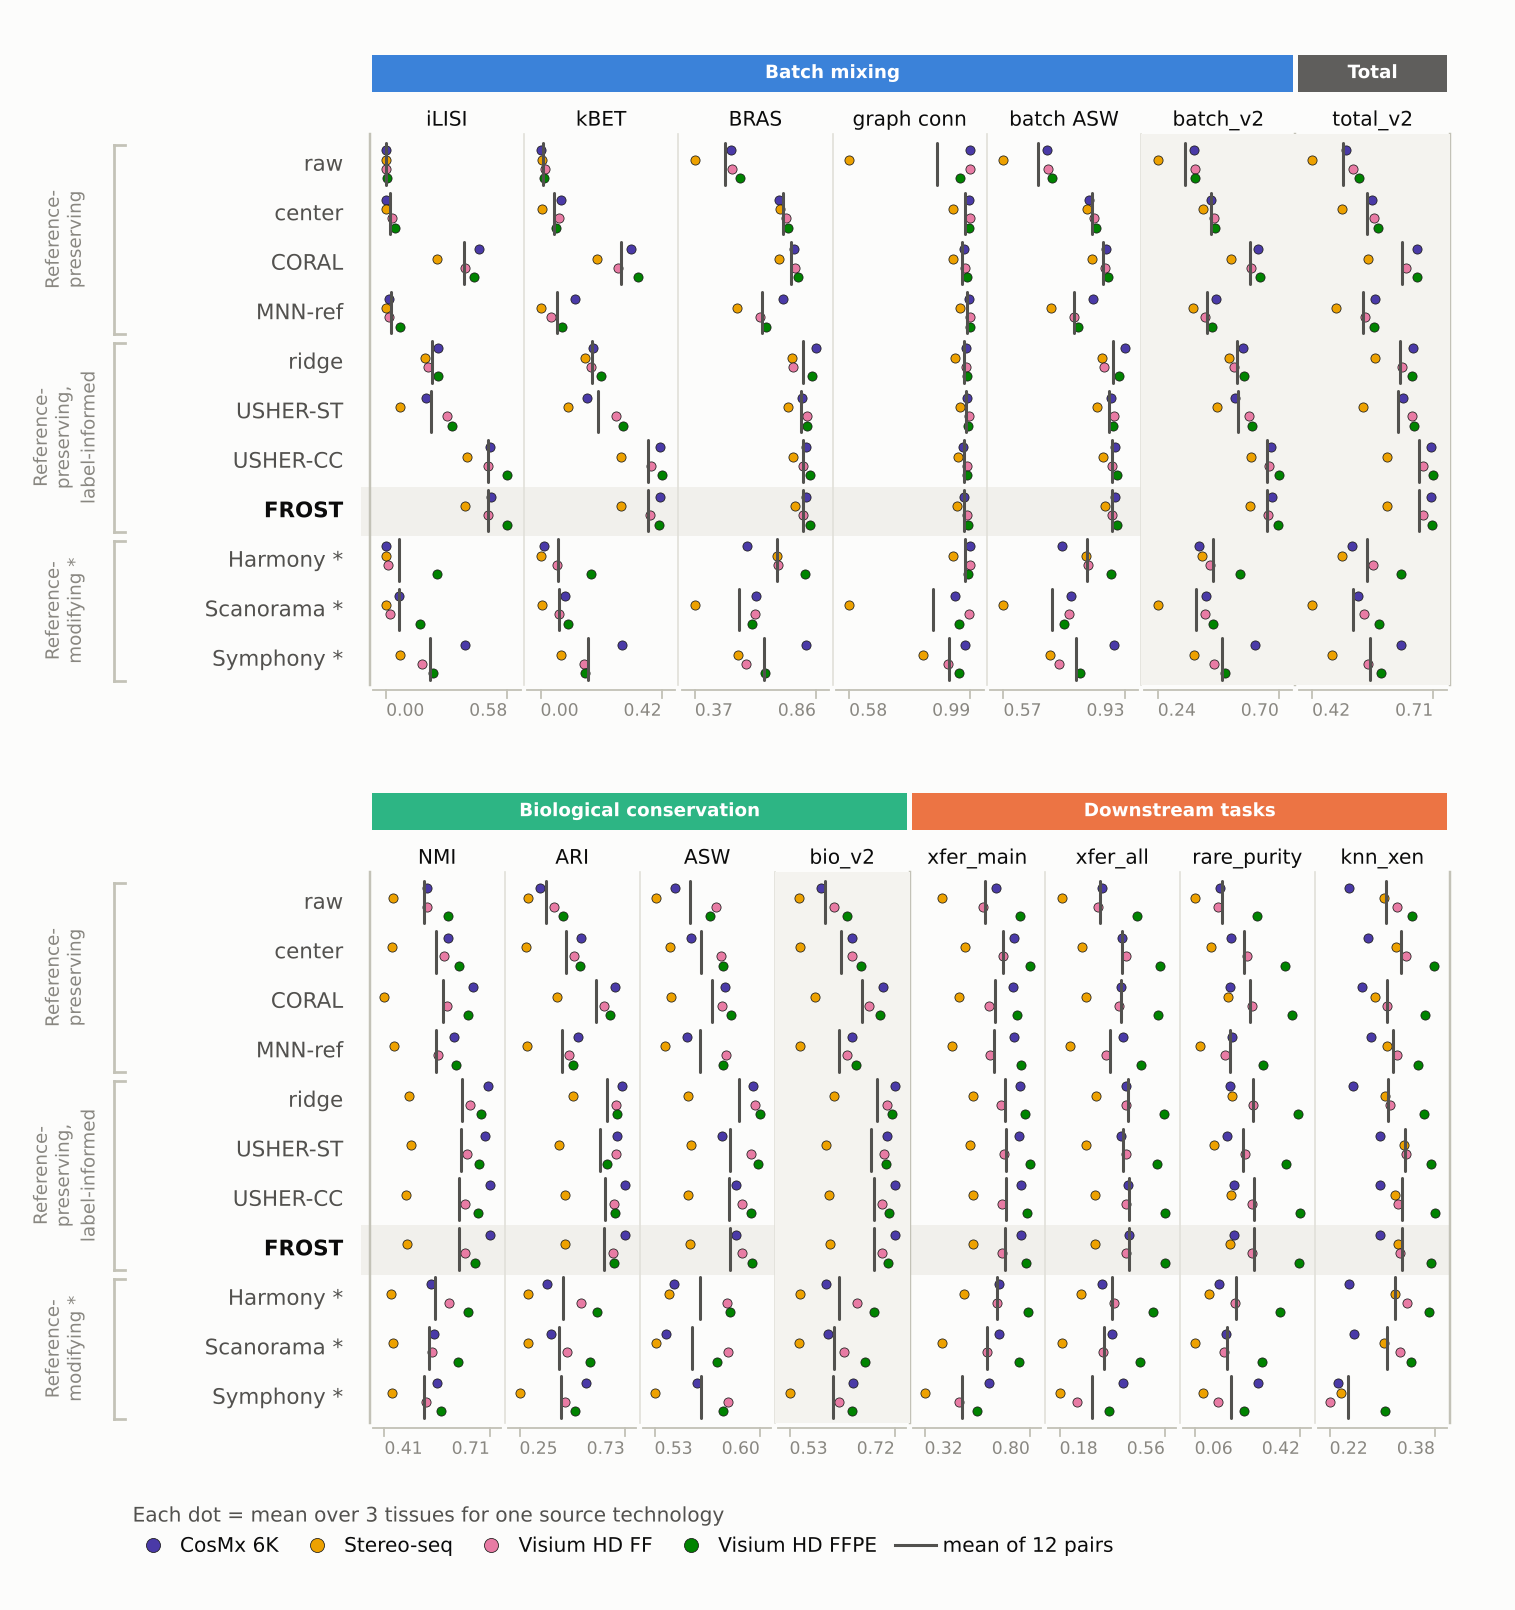
\includegraphics[width=\linewidth]{figs/fig_grid_tech.png}
\caption{All 16 metrics, 11 methods. Each dot is the mean over three tissues for one source technology; the vertical
bar is the mean over 12 pairs. Axes span the observed range of each metric, without min--max scaling across
methods. Shaded columns are group scores of the metrics to their left: batch\_v2 is the mean of iLISI, kBET, BRAS
and graph connectivity; bio\_v2 the mean of NMI, ARI, ASW, cLISI and isolated labels; total\_v2 $=0.4\,$batch\_v2
$+\,0.6\,$bio\_v2. $^{*}$Methods that modify the reference embedding. The four pairs of a tissue share a reference
and a patient, so the 12 pairs are not independent.}
\label{fig:grid}
\end{figure}

\begin{figure}[!t]
\centering
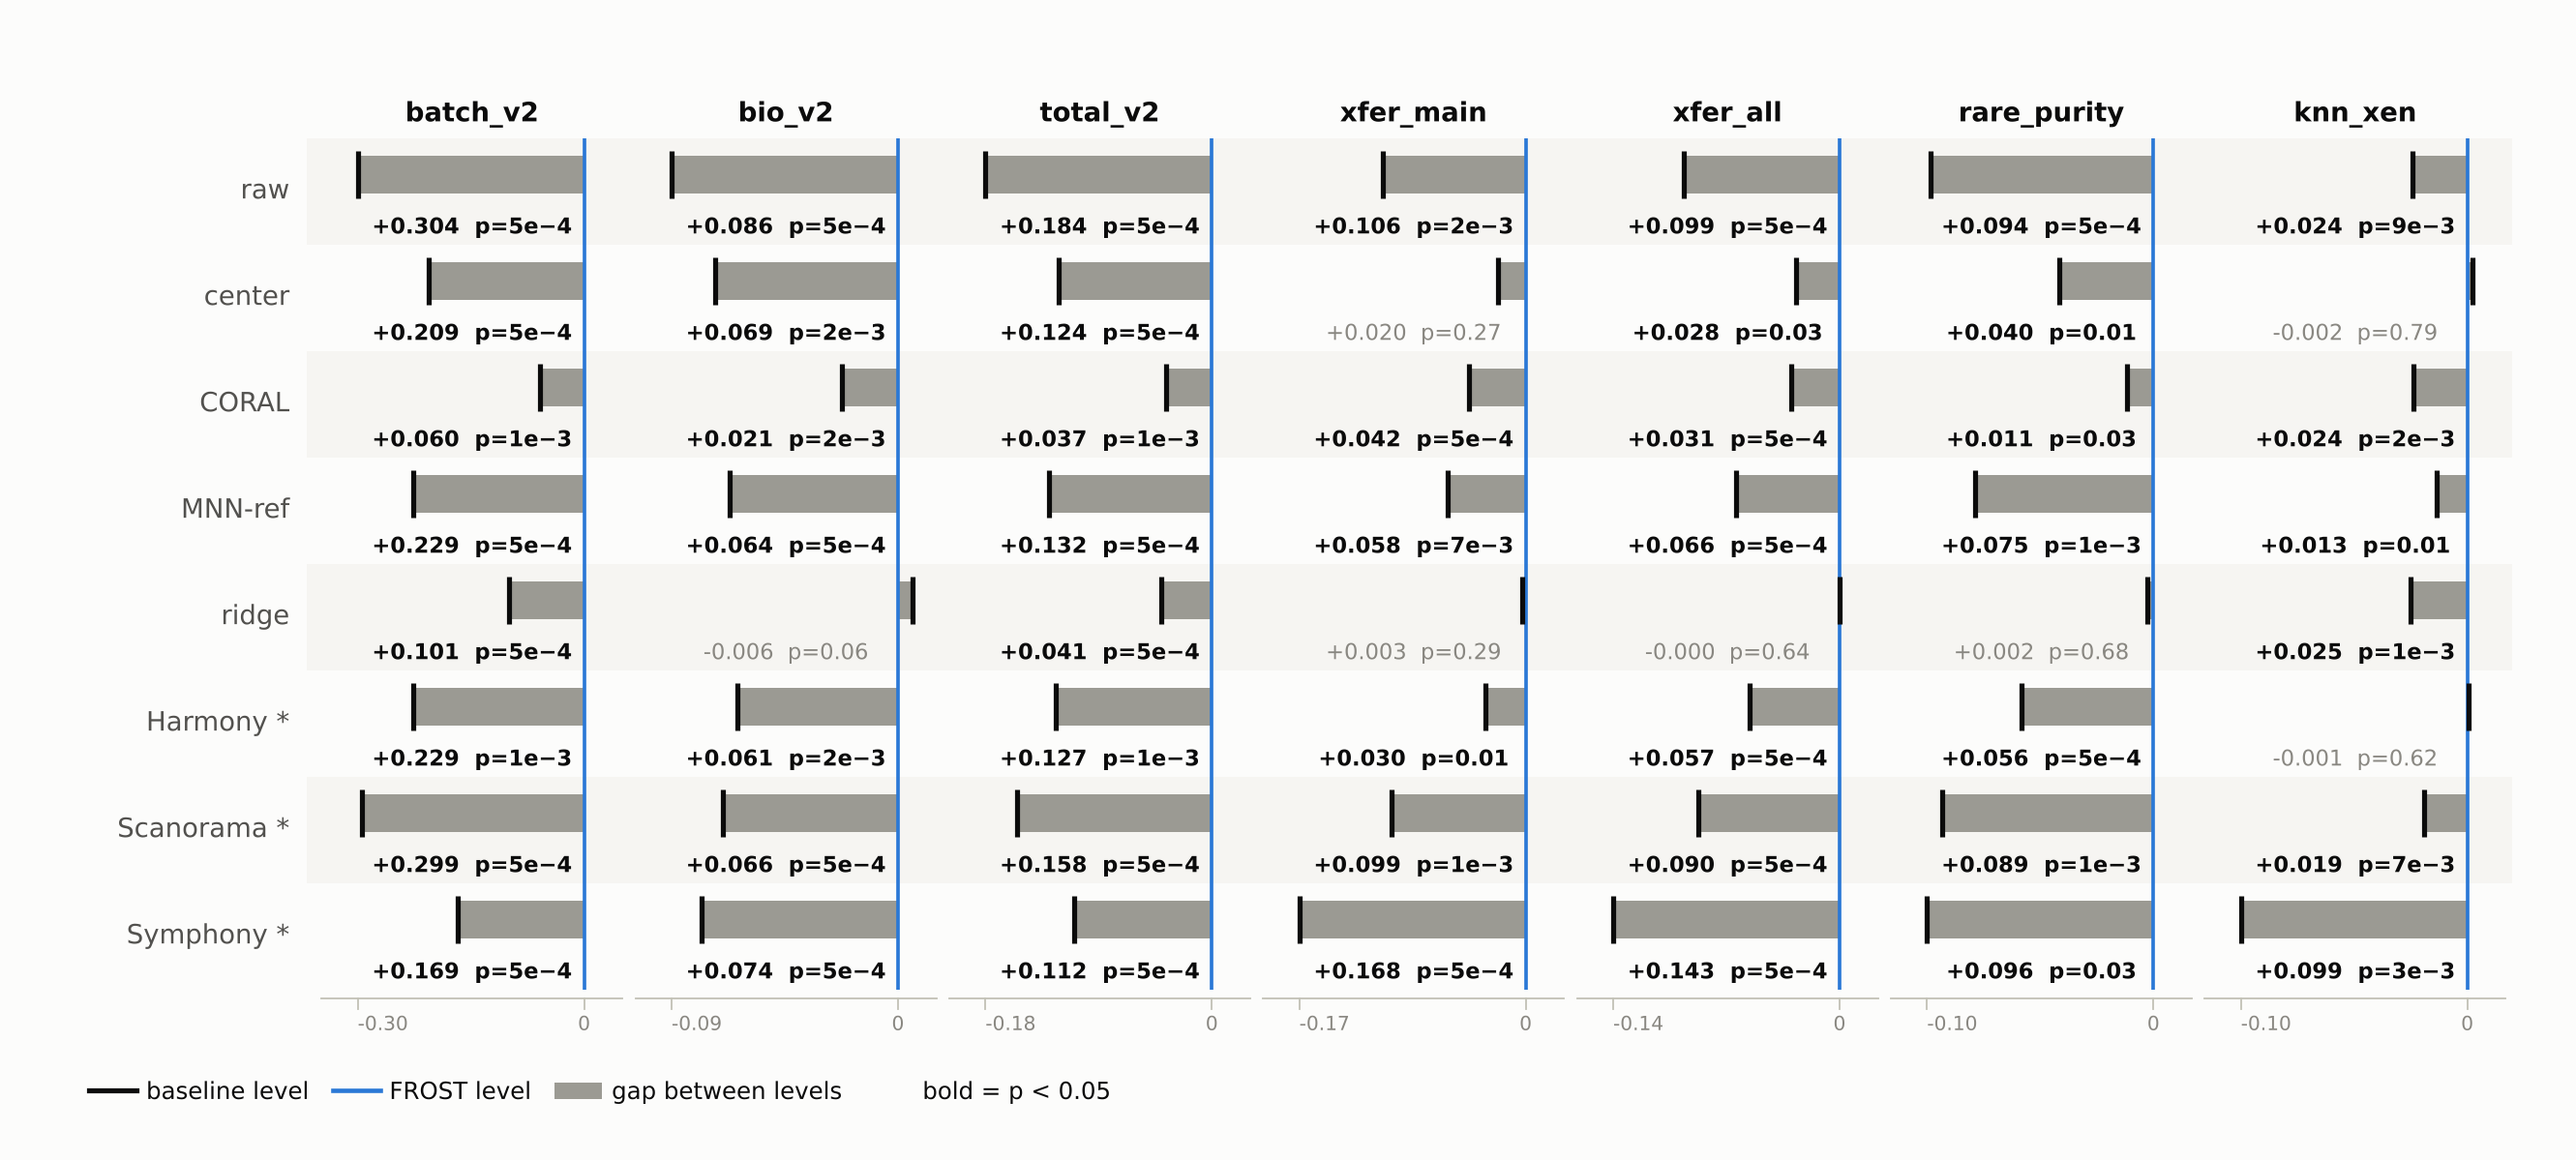
\includegraphics[width=\linewidth]{figs/fig_gaps.png}
\caption{Paired comparison of each baseline with \frost over 12 pairs. The blue line marks \frost; the black tick
marks the baseline, placed at minus the median of the 12 paired differences (\frost $-$ baseline). Bar, tick and
printed value all use that median, which is the quantity the Wilcoxon signed-rank test examines. Values in bold have
$p<0.05$. With 12 pairs $p$ cannot fall below $2/2^{12}\approx4.9\times10^{-4}$, and pairs within a tissue are
not independent, so $p$ describes consistency and the median describes magnitude. $^{*}$Methods that modify the
reference embedding.}
\label{fig:gaps}
\end{figure}

\subsection{Ablations}\label{sec:res_ablation}

\paragraph{Post-hoc moment matching.}\label{sec:res_coral}
On the common subsample, adding CORAL to USHER-ST (giving USHER-CC) raises mixing by $+0.191$ ($n=12$, $p=0.0015$)
and transfer by only $+0.0086$ (Table~\ref{tab:graphst}). On the main benchmark, \frost exceeds USHER-ST on
batch\_v2 ($p=0.0005$), total\_v2 ($p=0.0010$), xfer\_all ($p=0.0068$) and rare\_purity ($p=0.0024$), and does not
differ significantly on bio\_v2, xfer\_main or knn\_xen ($n=12$, except $n=11$ for xfer\_main). The two differ in
CORAL and in how the structure matrices are built; since the latter has no detectable effect (below), we attribute
the gain to CORAL. CORAL is thus justified on the cell-level metrics at no significant cost there. Its cost appears
at the gene level (Section~\ref{sec:limitations}).

\paragraph{Reference floor.}\label{sec:res_floor}
The per-class floor was fixed before evaluation, on a validation split of the training tiles. The rule was the
largest rare-type purity among floors that lost no more than 0.02 in xfer\_main or total score, with the 0.02
threshold set in advance. That rule chose 200. On held-out tiles, larger floors improve xfer\_main, xfer\_all and
rare-type purity slightly (Supplementary Table~\ref{tab:floor}), so 200 is conservative rather than tuned on
evaluation data.

\paragraph{Computational cost of the structure matrices.}\label{sec:res_cost}
Table~\ref{tab:cost} times three structure configurations on the four COAD pairs (seed 0, 25 EM iterations): the
adaptive landmark $\Cs$ of USHER-ST, a frozen exact $\Cs$ on the embeddings alone, and \frost's frozen exact $\Cs$
on augmented features. Freezing $\Cs$ cuts the number of $\Cs$ builds from 100 to 4, a 25-fold reduction equal
to the number of EM iterations. Each exact build is more expensive than a landmark one, but total $\Cs$ time still falls 2.7-fold,
and EM wall-clock time falls from 457.7\,s to 386.1\,s per pair. Adding the microenvironment block costs
nothing measurable (387.3\,s, with the same 8 builds). These diagnostic runs use 25 iterations, whereas the
benchmark maps use 10. The number of builds for the frozen configurations does not depend on the number of
iterations.

\begin{table}[t]
\centering
\caption{EM cost on the four COAD pairs (seed 0, 25 iterations). Wall-clock is real time. $\Cs$ time is thread
time summed over four worker threads; it is not real time and must not be added to wall-clock.}
\label{tab:cost}
\small
\begin{tabular}{@{}lccc@{}}
\toprule
 & landmark $\Cs$, recomputed & exact $\Cs$, frozen & \frost \\
\midrule
EM wall-clock, CosMx 6K (s)      & 431.7 & 355.4 & 361.7 \\
EM wall-clock, Visium HD FF (s)  & 462.0 & 404.5 & 385.8 \\
EM wall-clock, Visium HD FFPE (s)& 437.5 & 361.5 & 366.8 \\
EM wall-clock, Stereo-seq (s)    & 499.7 & 422.9 & 435.0 \\
EM wall-clock, mean (s)          & 457.7 & 386.1 & 387.3 \\
$\Cs$ builds                     & 100   & 4     & 4 \\
Total structure builds           & 104   & 8     & 8 \\
$\Cs$ thread time (s)            & 333.9 & 122.2 & 122.9 \\
\bottomrule
\end{tabular}
\end{table}

\paragraph{Structure matrices and the microenvironment term.}\label{sec:res_niche}
\frost and USHER-CC are indistinguishable on every metric: on the compact set, all $p\ge0.26$ ($n=12$), with no
median difference larger than 0.0008 in absolute value; on the common subsample, $p=0.75$ for transfer and $p=0.067$
for mixing. The difference measures the joint effect of three simultaneous changes to $\Cs$: adding the
microenvironment, replacing landmark distances with exact geodesics, and replacing per-iteration recomputation on
$f_\theta(\mathbf{X}^{s})$ with a single computation on the unmapped source. On the PCA pairs a fourth difference is
added: the 64-dimensional low-rank projection applies to the augmented features but not to the 50-dimensional
embeddings. We cannot separate the contribution of the microenvironment with the data at hand. What the frozen
construction does change is cost, as shown above.

\subsection{Comparison with USHER}\label{sec:res_usher}
Table~\ref{tab:usher} compares \frost with the unmodified USHER reference implementation on the four COAD pairs. With
four pairs and a single seed, no paired test can reach significance (exact two-sided floor $p=0.125$); we
therefore report differences descriptively. The two pipelines also differ in four components at once
(Table~\ref{tab:usher_vs_frost}), so this is a pipeline-level comparison, not an ablation.

The two methods sit at different points of the same trade-off, and their total scores are level (total\_v2 0.7055
for USHER, 0.7025 for \frost). USHER is higher on the mixing group score (batch\_v2 $-0.028$, \frost minus USHER);
\frost is higher on the conservation group score (bio\_v2 $+0.014$) and on every task metric, with the largest
differences on the three that probe rare types and local geometry: xfer\_all, rare-type purity and knn\_xen ($+0.034$ to $+0.038$). These are the metrics outside
USHER's own benchmark. Adding CORAL to USHER raises its mixing further without changing this pattern.

\frost reaches this point of the frontier at a fraction of the cost. USHER recomputes exact structure matrices
200 times per pair, against 8 for \frost ($2BT$ against $2B$ with $T=25$). USHER's EM took 2{,}570--3{,}219\,s per
pair (mean 2{,}911\,s), with 54--67\% spent building structure matrices. \frost took 361.7--435.0\,s (mean
387.3\,s) at the same number of iterations, about 7.5-fold less. Both ran on the same hardware type, but the timing
difference also includes the other three differences between the pipelines.

\begin{table}[t]
\centering
\caption{USHER reference implementation versus \frost, four COAD pairs. USHER: one seed, 25 iterations. \frost and
ridge: three seeds, means. The pipelines differ in four components (Table~\ref{tab:usher_vs_frost}). $\Delta$: \frost minus USHER. Imputation is
omitted because the archived values use the leaking protocol (Section~\ref{sec:limitations}).}
\label{tab:usher}
\small
\begin{tabular}{@{}llccccc@{}}
\toprule
Group & Metric & USHER & USHER + CORAL & \frost & ridge & $\Delta$ \\
\midrule
\multirow{6}{*}{Mixing}
 & iLISI        & 0.5551 & 0.6609 & 0.5261 & 0.2215 & -0.0290 \\
 & kBET         & 0.5153 & 0.5049 & 0.4440 & 0.1961 & -0.0713 \\
 & BRAS         & 0.8604 & 0.8387 & 0.8450 & 0.8502 & -0.0154 \\
 & graph conn.  & 0.9768 & 0.9747 & 0.9800 & 0.9796 & +0.0032 \\
 & batch ASW    & 0.9268 & 0.9147 & 0.9152 & 0.9196 & -0.0116 \\
 & batch\_v2    & 0.7269 & 0.7448 & 0.6987 & 0.5618 & -0.0282 \\
\midrule
\multirow{6}{*}{Conservation}
 & NMI          & 0.6411 & 0.6412 & 0.6780 & 0.6739 & +0.0369 \\
 & ARI          & 0.6442 & 0.6461 & 0.6828 & 0.6924 & +0.0386 \\
 & ASW          & 0.5924 & 0.5852 & 0.5826 & 0.5904 & -0.0098 \\
 & cLISI        & 0.9837 & 0.9891 & 0.9935 & 0.9939 & +0.0098 \\
 & iso.\ labels & 0.5950 & 0.5896 & 0.5884 & 0.5951 & -0.0066 \\
 & bio\_v2      & 0.6913 & 0.6902 & 0.7050 & 0.7091 & +0.0137 \\
\midrule
Total & total\_v2 & 0.7055 & 0.7120 & 0.7025 & 0.6502 & -0.0030 \\
\midrule
\multirow{4}{*}{Tasks}
 & xfer\_main   & 0.7052 & 0.6965 & 0.7090 & 0.7091 & +0.0038 \\
 & xfer\_all    & 0.4336 & 0.4405 & 0.4715 & 0.4663 & +0.0379 \\
 & rare\_purity & 0.2610 & 0.2803 & 0.2990 & 0.2909 & +0.0380 \\
 & knn\_xen     & 0.4119 & 0.4036 & 0.4456 & 0.4200 & +0.0337 \\
\bottomrule
\end{tabular}
\end{table}

\section{Scope and limitations}\label{sec:limitations}

\paragraph{Alignment trades gene-level fidelity for cell-level comparability.}
\frost fits a single global map so that source cells match the reference in distribution and in label
neighbourhoods. Nothing in that objective preserves the gene-expression neighbourhood of each individual cell, so
fine expression geometry is blurred. Four independent measurements show this, and the CORAL trade-off is the same
phenomenon at a smaller scale.
\begin{enumerate}
  \item \emph{Leakage-controlled imputation.} Standard baselines exceed every USHER-family variant, \frost included,
  in 11 of 12 pairs. Per-pair values were archived only for the three Stereo-seq pairs. There, no alignment exceeds
  \frost by a factor of 1.5, 1.6 and 4.9 (COAD, OV, HCC).
  \item \emph{Gene masking by fold}, run earlier on PCA embeddings only, ranked no alignment above centring above
  USHER on every pair it covered.
  \item \emph{Deconvolution} (below): centring is best, \frost wins no setting, and CORAL degrades most settings.
  \item \emph{Entropy of the deconvolution estimates} shows that USHER-family maps produce proportions that are too
  diffuse rather than too sharp.
\end{enumerate}
This is why we do not position \frost as a gene-level method. It is a scoping decision with a mechanism behind it,
not a failed task. The decision does not extend to alignment in general. Mutual-nearest-neighbour correction and
Harmony, which make local rather than global corrections, keep gene-level neighbourhoods about as well as no
alignment in the leakage-controlled protocol (COAD Stereo-seq: 0.2015 and 0.1792 against 0.1850). They also mix far
less: batch\_v2 is 0.463 and 0.522 on the four COAD pairs, against 0.699 for \frost and 0.378 without alignment.
The trade-off is therefore between how much a method mixes and how much gene-level structure it keeps, and the
reference-preserving global maps sit at the high-mixing end.

\paragraph{Why the original imputation protocol favoured \frost.}
In the original protocol, \frost ranks second (Table~\ref{tab:main}). A paradox shows that leakage is not the whole
story. Leakage alone would favour no alignment, whose source embedding, computed from all genes including the
predicted one, is left untouched. Yet no alignment scores low under that protocol (COAD Stereo-seq: 0.0945 against
0.1041 for \frost). The reason is that the original protocol predicts each gene from the 15 reference neighbours of
a mapped source cell. Without alignment those neighbours are meaningless, so the protocol rewards alignment and
leakage together. Because the map moves the very embedding that carries the leak, the two cannot be separated. The
reversed protocol queries reference cells, whose embedding is frozen and identical across reference-preserving
methods, and predicts from
mapped source neighbours. Leakage then cancels, and what remains is how much of the source's gene-level neighbourhood
structure survives the map. No alignment preserves all of it. Two independent leakage controls---the reversed
protocol and gene masking---agree. We have not tested the reversed protocol for artefacts of its own, and the
decisive experiment, gene masking by fold on scGPT-spatial embeddings, was not run.

\paragraph{The cell-level results are unaffected.}
The seven compact metrics and the comparison with GraphST are computed from labels and from geometry in the frozen
reference space. They involve no gene prediction, so they have no leakage channel. Every significant difference in
Section~\ref{sec:results} is independent of the issue above.

\paragraph{Cell-type deconvolution.}
We did not position \frost as a deconvolution method, and the boundary is architectural rather than empirical:
reference-based deconvolution consumes counts against a gene-by-cell-type signature matrix and rests on the
additivity of mRNA ($\mathbf{y}\approx\mathbf{S}\mathbf{w}$), whereas \frost emits embeddings with no gene axis,
no preserved expression scale and no additivity. We nonetheless asked the narrower question of whether alignment
helps a \emph{neighbour-based} proportion estimator, using pseudo-spots of $k=4$ and $k=8$ nearest cells. Their
median enclosing diameters are 49--65\um and 91--124\um, bracketing the 55\um Visium spot. We tested 11 technology
pairs at both spot sizes (22 settings). Alignment does not help. Simple centring is the only method never worse
than the prior-composition floor (mean JSD 0.0855 against 0.1242 for \frost, which wins no setting; $p=0.001$).
Post-hoc CORAL degrades 16 of 22 settings on both JSD and Pearson correlation. We therefore report only the
narrow claim, and note that count-based models such as RCTD~\citep{cable2022rctd} and
cell2location~\citep{kleshchevnikov2022cell2location} were not evaluated. The CORAL result matters in its own right,
because it quantifies a trade-off of our best-performing configuration: CORAL buys $+0.191$ in batch mixing
($p=0.0015$) for $+0.0086$ in label transfer, at a measurable cost in local density fidelity.

\paragraph{The microenvironment term.}
Its contribution cannot be separated from that of freezing exact structure matrices
(Section~\ref{sec:res_niche}). On the gene level, it recovers part of the loss described above on one pair: under
the reversed protocol, \frost exceeds USHER-CC by $+0.044$ on COAD Stereo-seq, with disjoint bootstrap intervals,
yet still falls short of no alignment. A microenvironment-only variant was run with a single seed. The 15-neighbour
radius ranges from 16.7\um (Visium HD FF) to 33.9\um (CosMx), so the two structure matrices compare neighbourhoods
at different physical scales.

\paragraph{Scope of the evaluation.}
SPATCH provides three patients per tissue; we used one, so the 12 pairs come from three patients and share a
reference within each tissue. Paired tests describe consistency across these pairs, not generalisation across
patients. The most informative extension would be the Stereo-seq pairs of the remaining patients. Only one spatially
aware baseline was run, at its published defaults, with one seed and on a subsample; STAligner could not be
installed. Harmony and Scanorama were fitted transductively on held-out tiles, which favours them. The USHER
reference implementation was run with one seed on four pairs. Timings come from diagnostic runs at 25 iterations;
peak memory was not measured.

\section{Conclusion}\label{sec:conclusion}
Integrating platforms into a fixed reference changes which methods work: a spatially aware joint method transfers labels worse than no alignment here and rebuilds
the reference it was asked to serve. \frost keeps the reference fixed by construction, transfers labels at least as
well as every baseline, and sits on the mixing--conservation frontier with 25-fold fewer structure computations than
the algorithm it builds on; gene-level information remains outside the reach of embedding alignment.

\paragraph{Code availability.} Code will be made available.


\bibliographystyle{plainnat}
\bibliography{refs}

\end{document}
